\documentclass[12pt]{article}
\usepackage{amsmath}
\usepackage{amssymb}
\usepackage{amsthm}
\usepackage{amsfonts}
\usepackage{algpseudocode}
\usepackage{algorithm}
\usepackage{mathrsfs}
\usepackage{graphicx}
\usepackage{times}
\usepackage{color}
\usepackage{appendix}
\usepackage{subfigure}
\usepackage{enumerate}
\usepackage{mathtools}
\usepackage{multirow}
\usepackage{booktabs}
\numberwithin{table}{section}
\usepackage{enumitem} %change list depth

\usepackage{listings}
\usepackage{xcolor}

\definecolor{codegreen}{rgb}{0,0.6,0}
\definecolor{codegray}{rgb}{0.5,0.5,0.5}
\definecolor{codepurple}{rgb}{0.58,0,0.82}
\definecolor{backcolour}{rgb}{0.95,0.95,0.92}

\lstdefinestyle{mystyle}{
	backgroundcolor=\color{backcolour},   
	commentstyle=\color{codegreen},
	keywordstyle=\color{magenta},
	numberstyle=\tiny\color{codegray},
	stringstyle=\color{codepurple},
	basicstyle=\ttfamily\footnotesize,
	breakatwhitespace=false,         
	breaklines=true,                 
	captionpos=b,                    
	keepspaces=true,                 
	numbers=left,                    
	numbersep=5pt,                  
	showspaces=false,                
	showstringspaces=false,
	showtabs=false,                  
	tabsize=2
}

\lstset{style=mystyle}

\usepackage{tikz}
\usetikzlibrary{positioning}
\usetikzlibrary{arrows,arrows.meta}
\setlistdepth{8}
\renewlist{itemize}{itemize}{8}

\newcommand{\question}[2][]{\begin{flushleft}
		\Large\textbf{Question #1}: \large\textit{#2}
		
\end{flushleft}}
\newcommand{\sol}{\textbf{Solution}:} %Use if you want a boldface solution line
\newcommand{\maketitletwo}[2][]{\begin{center}
		\Large{\textbf{Homework #1}
			
			ECE 590: Towards More Reliable Software} % Name of course here
		\vspace{5pt}
		
		\normalsize{Jeff Fan  \hspace{1em} $\left|\right|$ \hspace{1em}zf70@duke.edu  % Your name here
			
			\today}        % Change to due date if preferred
		\vspace{15pt}
		
\end{center}}

\begin{document}
	\maketitletwo[5]  % Optional argument is assignment number
	%Keep a blank space between maketitletwo and \question[1]
	
	\section*{Question 1: } 
	
	\textbf{Laplace Trend Test results.}

	\begin{lstlisting}[language=R]
library(ggplot2)

calculateAndPlotLaplaceTrend <- function(dataFrame, dataSetName) {
	# Initialize the results matrix
	resultsMatrix <- matrix(nrow = nrow(dataFrame), ncol = 2)
	
	# Calculation loop
	for (index in 2:nrow(dataFrame)) {
		# Calculate the trend value
		cumulativeSum <- sum(dataFrame[1:index, 2])
		# Calculate the partial cumulative sum
		partialCumulativeSum <- sum(sapply(2:(index-1), function(m) sum(dataFrame[1:m, 2])))
		# Store the trend value in the results matrix
		resultsMatrix[index, 2] <- ((1/(index-1))*partialCumulativeSum - cumulativeSum/2)/(cumulativeSum*sqrt(1/(12*(index - 1))))
	}
	
	# Define filename for plots
	generatePlotFilename <- function(extension) paste0(dataSetName, "_LaplaceTrend.", extension)
	
	# Save plot as EPS to be used in LaTeX
	postscript(generatePlotFilename("eps"), horizontal = FALSE, onefile = FALSE, paper = "special", height = 6, width = 6)
	generatePlot(resultsMatrix, dataSetName)
	dev.off()
	
	# Save plot as PNG for human viewing
	png(generatePlotFilename("png"), width = 480, height = 480)
	generatePlot(resultsMatrix, dataSetName)
	dev.off()
}

generatePlot <- function(trendResults, titleName) {
	plot(1:nrow(trendResults), trendResults[, 2], type = "o", col = "blue", xlab = "Index", ylab = "Trend Value",
	main = paste("Laplace Trend Test for", titleName))
	abline(h = c(1.96, -1.96), col = "gray60")
}

data1 <- read.csv("../data1.csv")
data2 <- read.csv("../data2.csv")

# Perform the calculation and plotting for each dataset
calculateAndPlotLaplaceTrend(data1, "Data1")
calculateAndPlotLaplaceTrend(data2, "Data2")\end{lstlisting} 
\begin{center}
	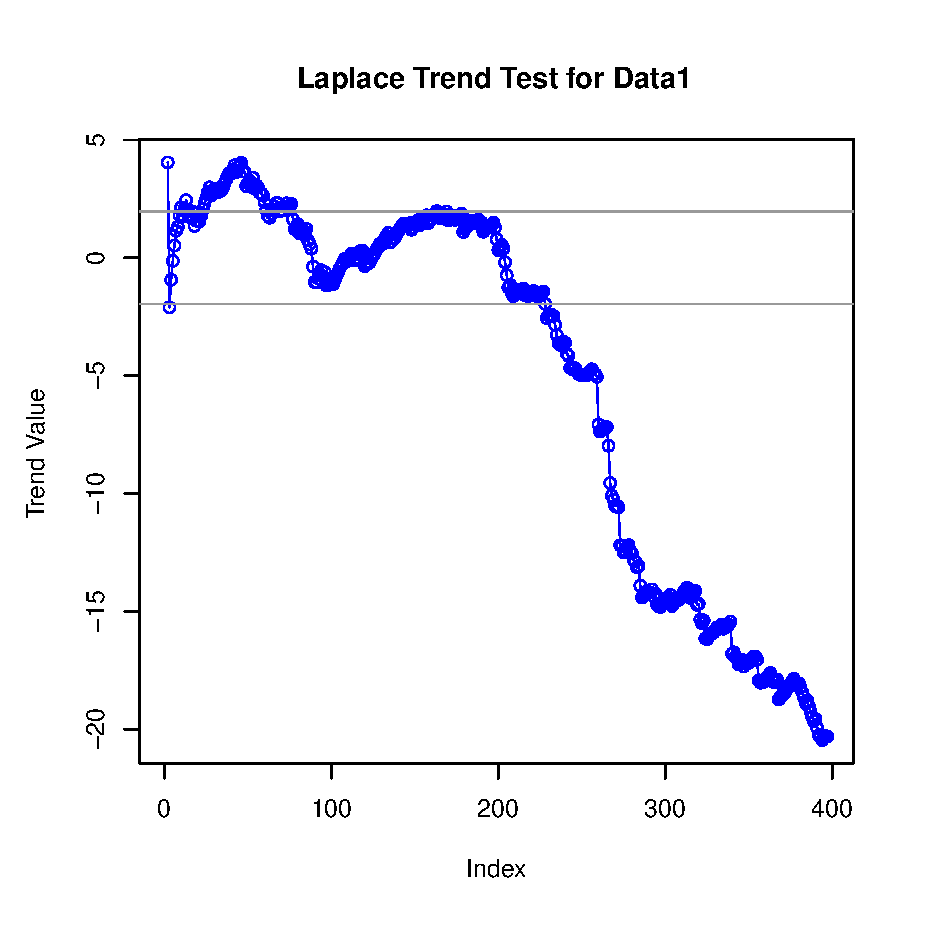
\includegraphics[width=0.5\textwidth]{image/Data1_LaplaceTrend.eps}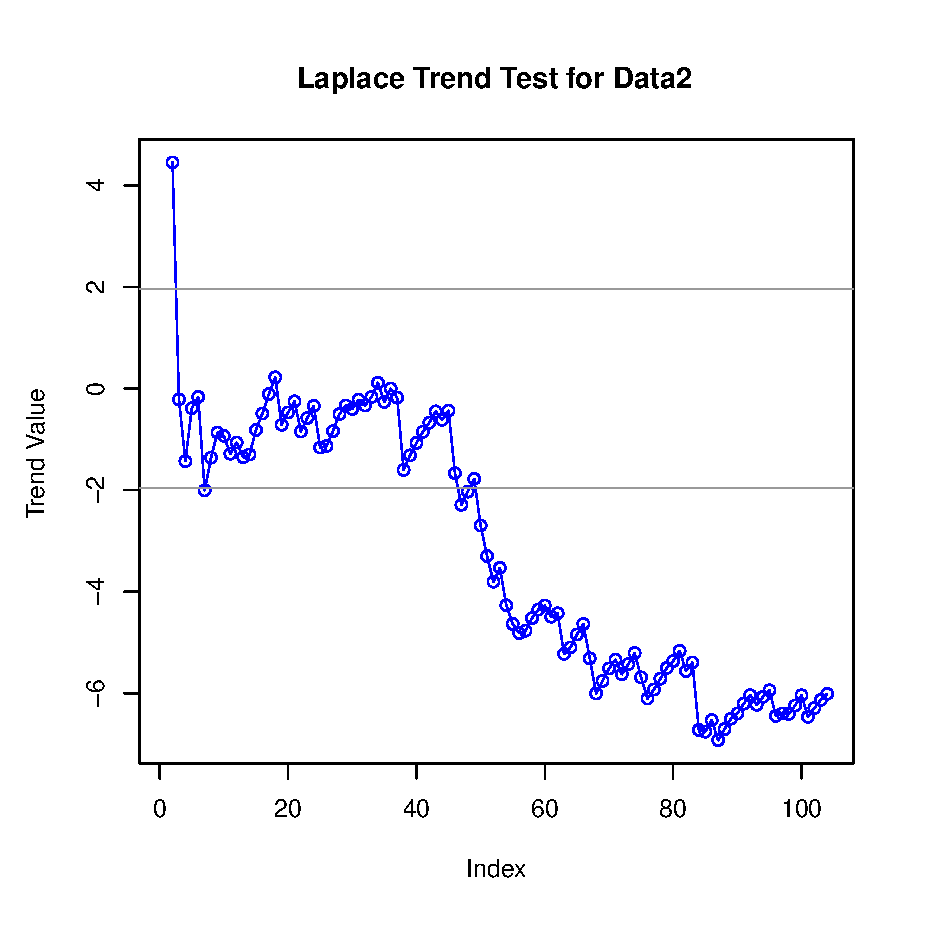
\includegraphics[width=0.5\textwidth]{image/Data2_LaplaceTrend.eps}
	
	{\small Fig. 1. Laplace Trend Test result of data1.}
	{\small Fig. 2. Laplace Trend Test result of data2.}
\end{center}

The provided calculateAndPlotLaplaceTrend function and its helper generatePlot are designed to perform a Laplace trend test on a given dataset and visualize the results. The Laplace trend test is a statistical method used to identify trends within a dataset, which can be particularly useful in time series analysis.

The formula used for calculating the trend value at each index incorporates both the cumulative sum and the partial cumulative sum. It is designed to normalize the trend measure, making it easier to compare across different points in time or across datasets. The normalization factor includes the square root of 1/(12*(index - 1)), which adjusts for the size of the data sample and helps to stabilize the variance.

Horizontal lines at 1.96 and -1.96 (abline(h = c(1.96, -1.96), col = "gray60")) are drawn to provide a reference for statistical significance, assuming a normal distribution of trend values. These lines correspond to approximately the 95\% confidence interval for a two-tailed test, where values outside this range might indicate a significant trend.

The calculateAndPlotLaplaceTrend function and its helper generatePlot provide a means to quantitatively assess and visualize trends within datasets. The choice of calculation method and visualization parameters are designed to offer a clear, standardized approach to trend analysis. This can be particularly useful in exploratory data analysis, where identifying and understanding trends is a key step in forming hypotheses about the data.\\
\\

	\textbf{2. SRGMs fitting results}
	
	\begin{lstlisting}[language=R]
library(Rsrat)
failureData <- read.csv(file = "data1.csv", header = TRUE)
nhppModelFit <- fit.srm.nhpp(te = 1000, time = failureData$Time.to.Failure, selection = NULL)

png("data1.png", width = 480, height = 480)
mvfplot(te = 1000, time = failureData$Time.to.Failure, srms = nhppModelFit)
dev.off()

png("data1_lambda.png", width = 480, height = 480)
plot(1:100000,nhppModelFit$exp$srm$intensity(1:100000),lty=1)
lines(1:100000,nhppModelFit$exp$srm$intensity(1:100000),lty=1)
lines(1:100000,nhppModelFit$gamma$srm$intensity(1:100000),lty=1)
lines(1:100000,nhppModelFit$pareto$srm$intensity(1:100000),lty=1)
lines(1:100000,nhppModelFit$tnorm$srm$intensity(1:100000),lty=1)
lines(1:100000,nhppModelFit$lnorm$srm$intensity(1:100000),lty=1)
lines(1:100000,nhppModelFit$tlogis$srm$intensity(1:100000),lty=1)
lines(1:100000,nhppModelFit$llogis$srm$intensity(1:100000),lty=1)
lines(1:100000,nhppModelFit$txvmax$srm$intensity(1:100000),lty=1)
lines(1:100000,nhppModelFit$lxvmax$srm$intensity(1:100000),lty=1)
lines(1:100000,nhppModelFit$txvmin$srm$intensity(1:100000),lty=1)
lines(1:100000,nhppModelFit$lxvmin$srm$intensity(1:100000),lty=)
dev.off()\end{lstlisting} 

\begin{center}
	\includegraphics[width=0.5\textwidth]{image/data1.eps}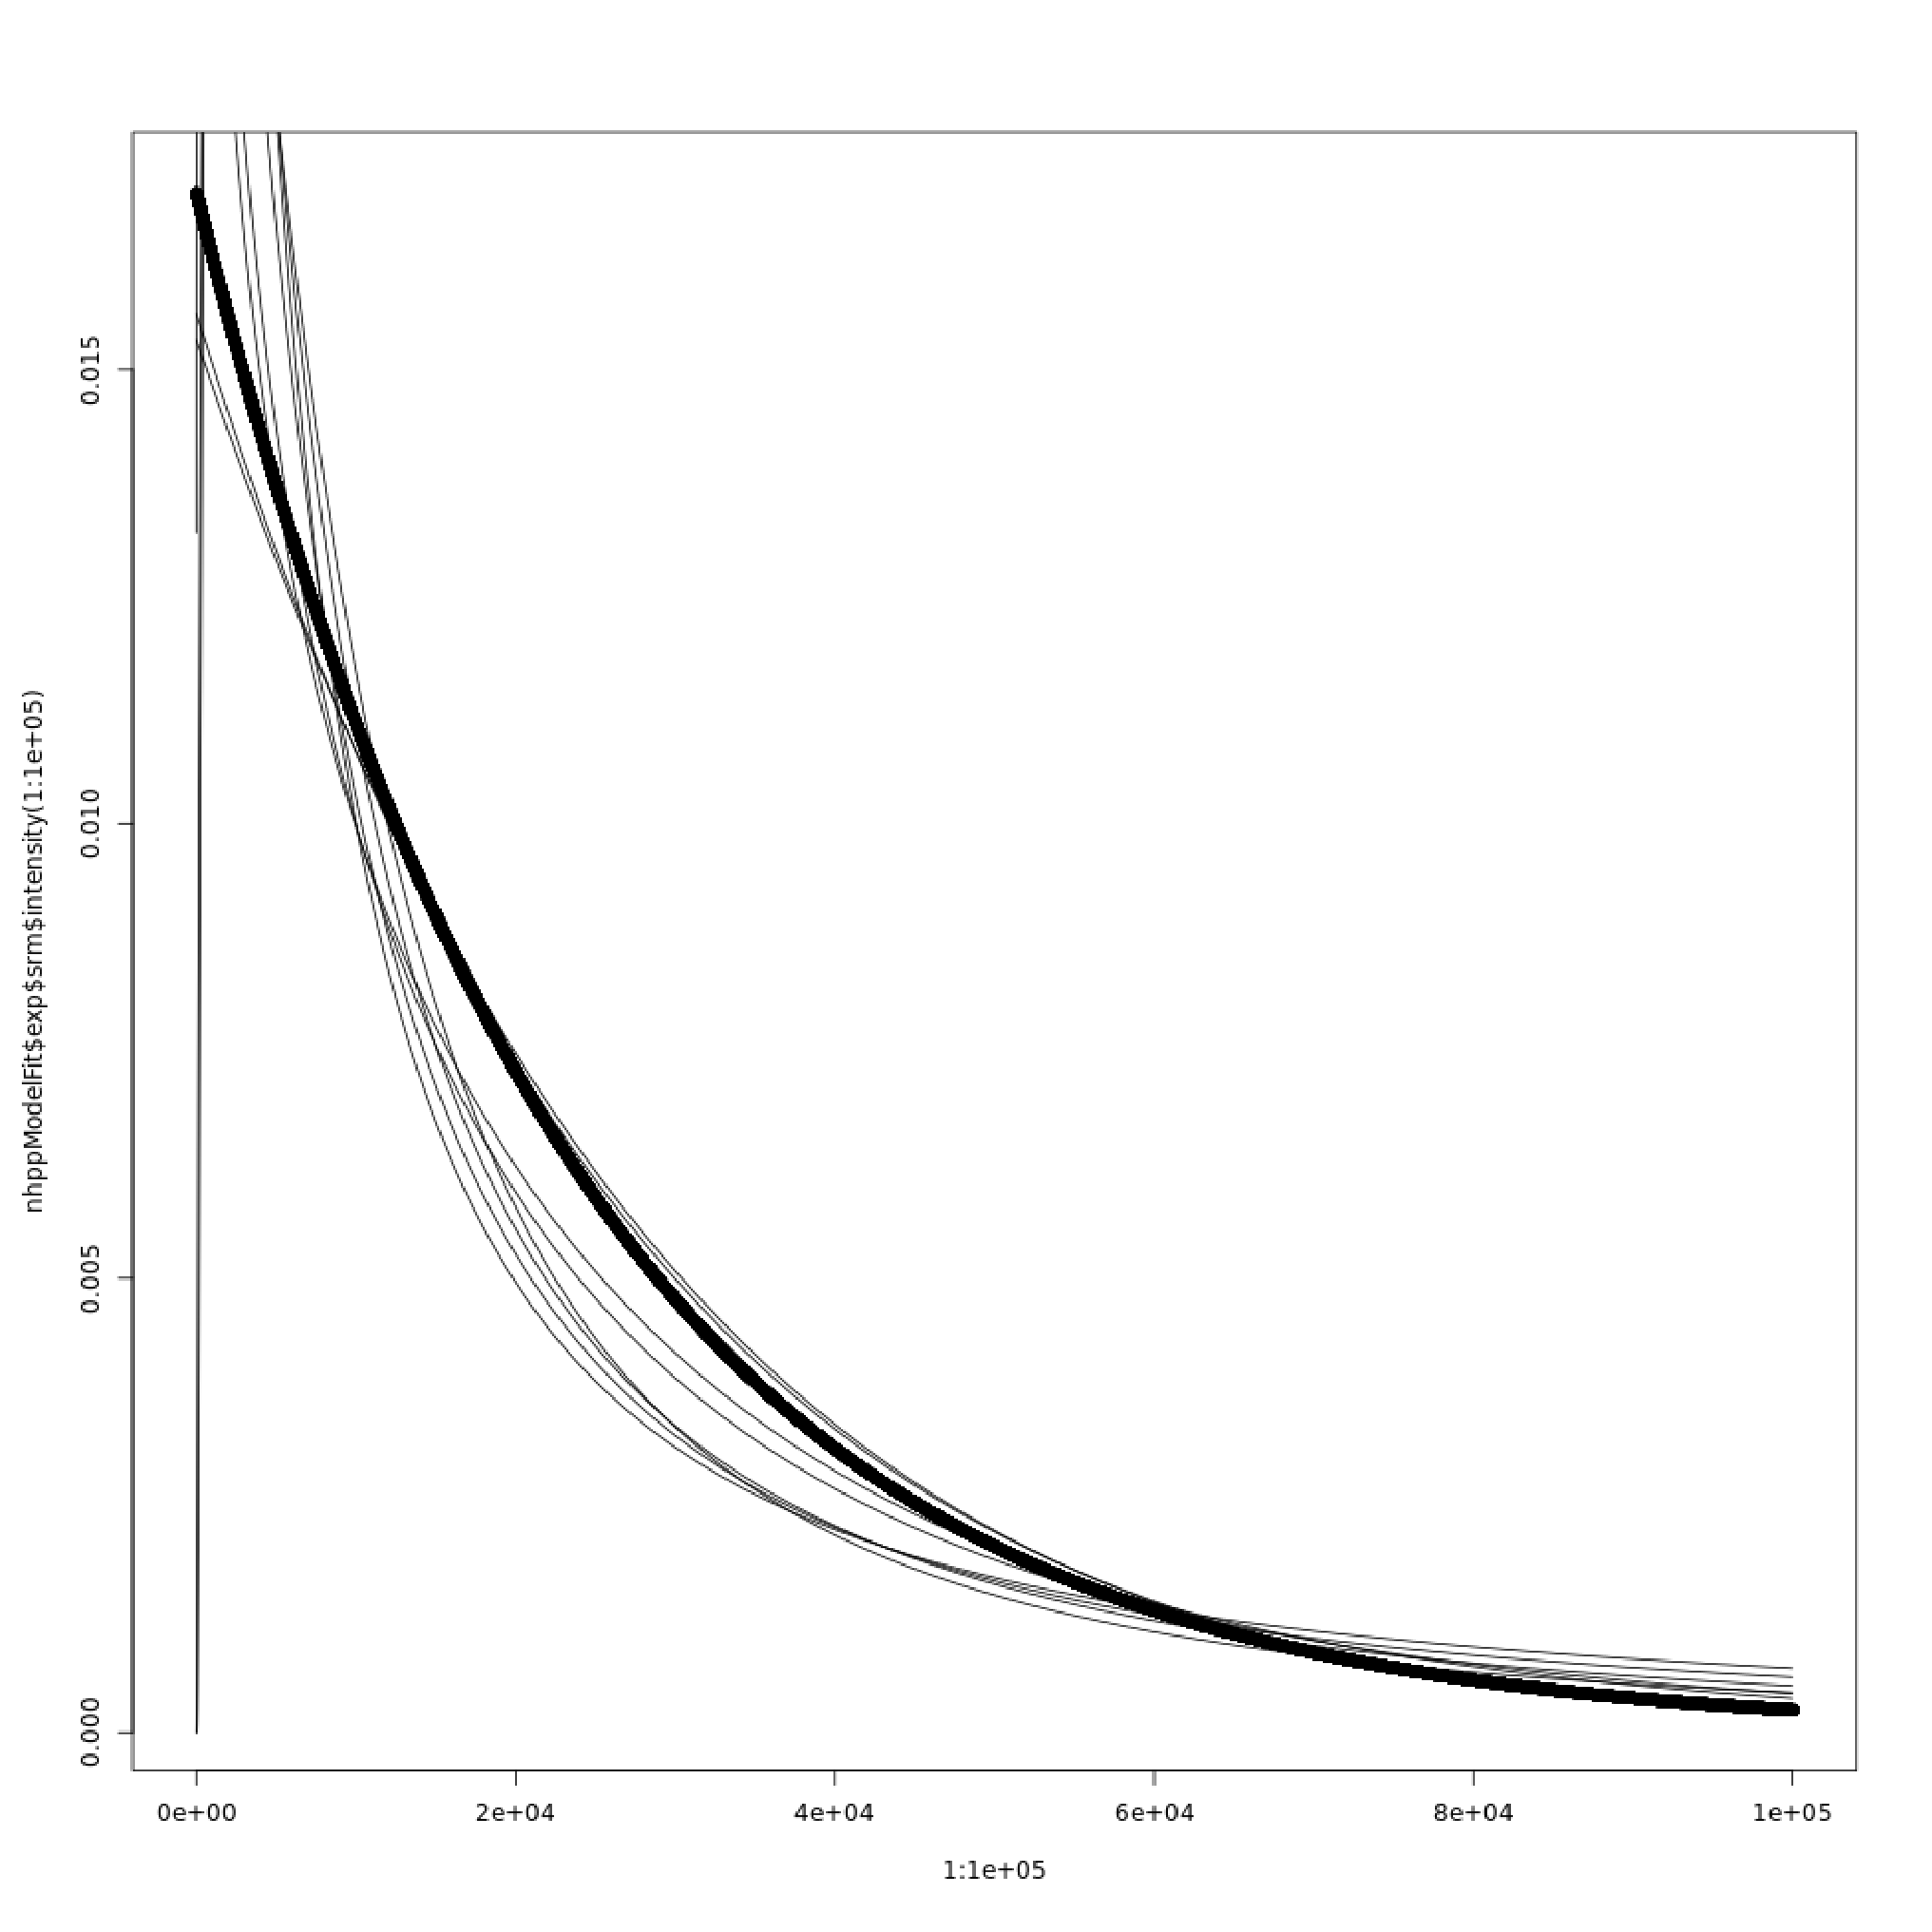
\includegraphics[width=0.5\textwidth]{image/data1_lambda.eps}
	
	{\small Fig. 3. Original m(t) and fitted m(t) of data1.}
	{\small Fig. 4. Lambda curves of data1.}
\end{center}

\begin{lstlisting}[language=R]
	library(Rsrat)
	failureData <- read.csv(file = "data2.csv", header = TRUE)
	nhppModelFit <- fit.srm.nhpp(te = 1000, time = failureData$Time.to.Failure, selection = NULL)
	
	png("data2.png", width = 480, height = 480)
	mvfplot(te = 1000, time = failureData$Time.to.Failure, srms = nhppModelFit)
	dev.off()
	
	png("data2_lambda.png", width = 480, height = 480)
	plot(1:100000,nhppModelFit$exp$srm$intensity(1:100000),lty=1)
	lines(1:100000,nhppModelFit$exp$srm$intensity(1:100000),lty=1)
	lines(1:100000,nhppModelFit$gamma$srm$intensity(1:100000),lty=1)
	lines(1:100000,nhppModelFit$pareto$srm$intensity(1:100000),lty=1)
	lines(1:100000,nhppModelFit$tnorm$srm$intensity(1:100000),lty=1)
	lines(1:100000,nhppModelFit$lnorm$srm$intensity(1:100000),lty=1)
	lines(1:100000,nhppModelFit$tlogis$srm$intensity(1:100000),lty=1)
	lines(1:100000,nhppModelFit$llogis$srm$intensity(1:100000),lty=1)
	lines(1:100000,nhppModelFit$txvmax$srm$intensity(1:100000),lty=1)
	lines(1:100000,nhppModelFit$lxvmax$srm$intensity(1:100000),lty=1)
	lines(1:100000,nhppModelFit$txvmin$srm$intensity(1:100000),lty=1)
	lines(1:100000,nhppModelFit$lxvmin$srm$intensity(1:100000),lty=)
	dev.off()\end{lstlisting} 

\begin{center}
	\includegraphics[width=0.5\textwidth]{image/data2.eps}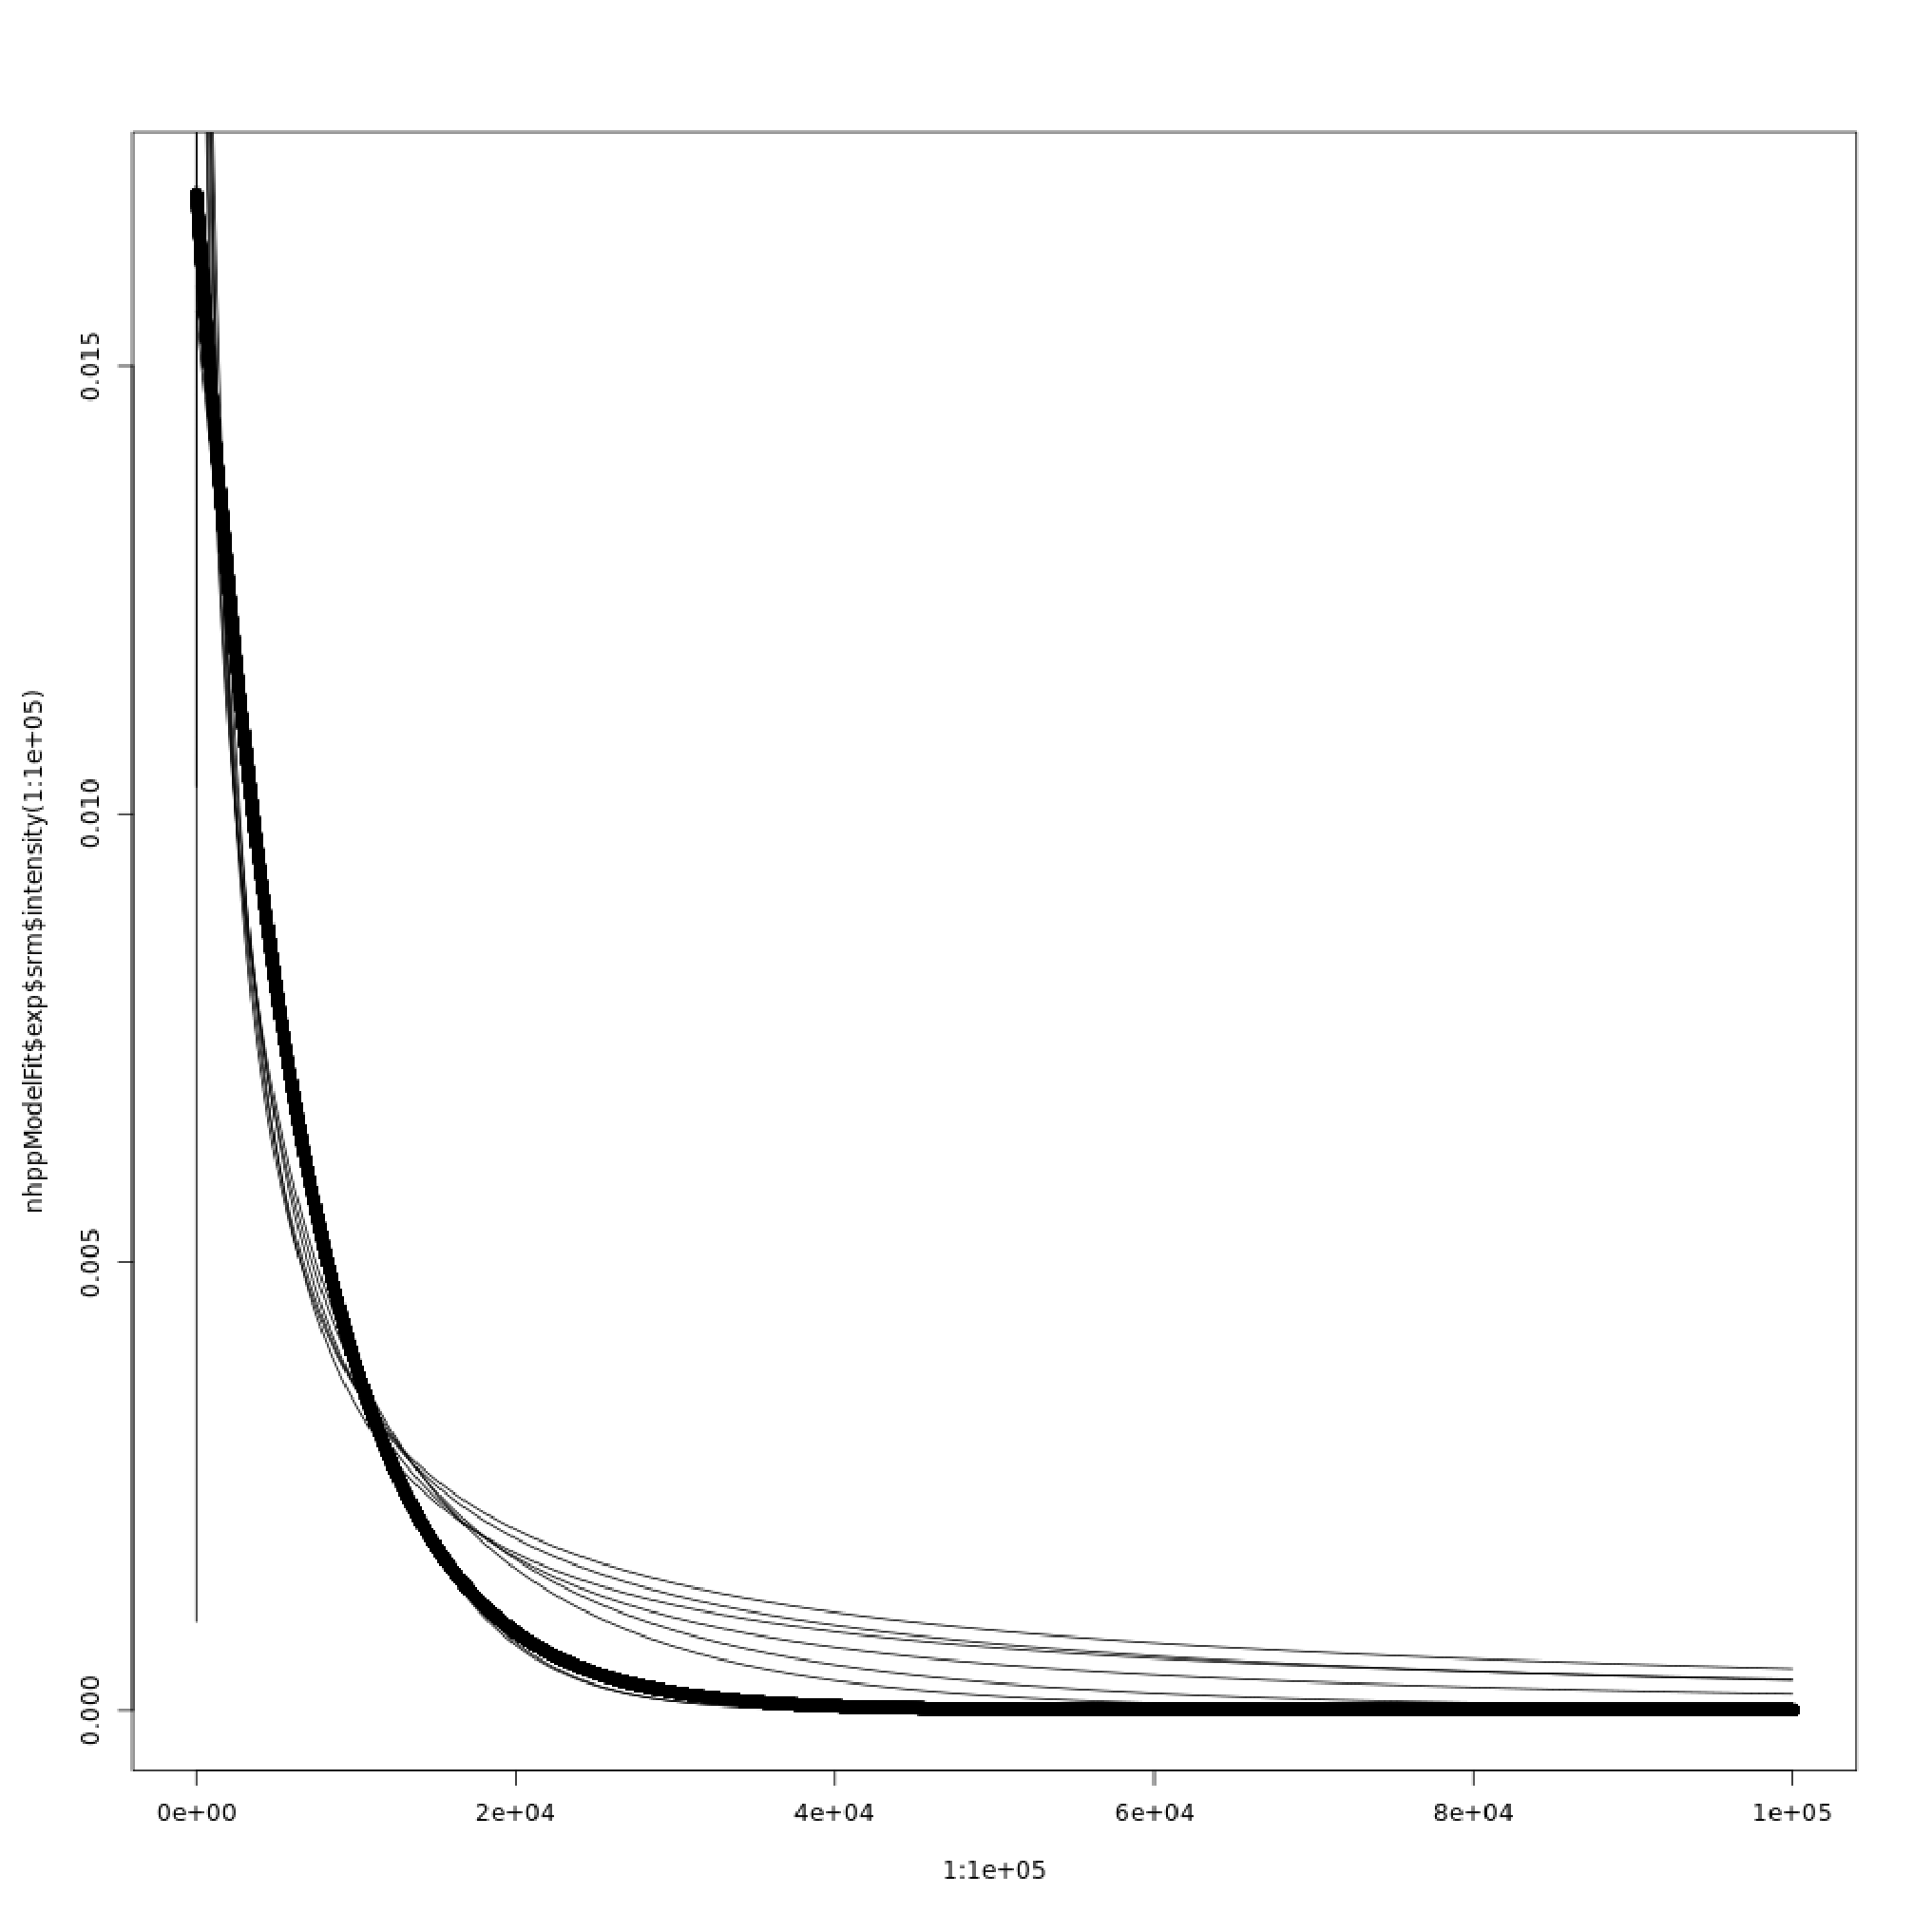
\includegraphics[width=0.5\textwidth]{image/data2_lambda.eps}
	
	{\small Fig. 5. Original m(t) and fitted m(t) of data2.}
	{\small Fig. 6. Lambda curves of data2.}
\end{center}


The above code snippet utilizes the Rsrat package in R to fit a Non-Homogeneous Poisson Process (NHPP) software reliability model to failure data, and then generates plots to visualize both the Mean Value Function (MVF) and the failure intensity function (Lambda) derived from the fitted model.

The fit.srm.nhpp function from the Rsrat package is used to fit an NHPP model to the time-to-failure data. This function selects an appropriate NHPP model based on the data and calculates the parameters of that model. The choice of te = 1000 indicates the end time for model fitting, providing a boundary for the data considered in the model.

A custom plot of the failure intensity function (Lambda) for different models is generated. The failure intensity function describes the rate at which failures are expected to occur at any given time. This plot visualizes how the expected failure rate changes over time under different statistical models fitted to the data.

The choice to plot the failure intensity function over 1:100000 is a decision to cover a wide range of time, ensuring that the behavior of the failure intensity function is captured across the entire lifecycle of the system or product being modeled. This range should be adjusted based on the specific time frame of interest and the distribution of failure times in the dataset.

\end{document}
